\documentclass[8pt,aspectratio=169]{beamer}
\usepackage{poly}
\usepackage{subcaption}
\usepackage{animate}

% ================================================================================
% Metadata
% ================================================================================

\title{Introduction to Moreau's Sweeping\\ Process}
\subtitle{EE6431 Course project}
\author{Done by : S.Janarthanan, EE21B060}
\institute[COMP]{IIT Madras}
\date{May 3, 2025}

% ================================================================================
% Main Body
% ================================================================================

\begin{document}
\maketitle % generate the title slide

\section{Introduction and motivation}

\begin{frame}{Introduction - what is a sweeping process?}
    \begin{itemize}
        \item The sweeping process is a class of differential inclusions, which were first introduced by the French mathematician Jean-Jacques Moreau in the 1970s.
        \item Originally intended to model elastoplastic systems, it has since found many applications in in diverse areas, such as nonsmooth electrical and mechanical systems, crowd motion, hysteresis phenomena etc.
        \item The sweeping process deals with differential inclusions of the form :
            \begin{equation*}
                \dot{x}(t) \in -N(C(t); x(t)),
            \end{equation*}
            where $C(t)$ is a time varying set, and $N(S; p)$ denotes the outward normal cone to the set $S$ at point $p$.
        \item The survey presentation, written by Emilio Vilches, explores some real life systems that are modeled by the sweeping process and broadly talks about existence of solutions to such systems.
    \end{itemize}
\end{frame}


\begin{frame}{Motivation and interpretation}
    \begin{itemize}
        \item Consider a closed, time varying set $C(t)$, and a point $x(t)$ inside it. Let us say the point $x(t)$ wants to always stay in the set $C(t)$ - so when the set $C$ moves, our point $x$ has to move along with it, so that it is not left behind.
        \item One of the geometric motivations we'd seen for the normal cone at a point was that it roughly represented the \textbf{most efficient directions to leave the set}. Naturally, the most efficient way for our point to ensure that it stays in the set $C(t)$ would be the move opposite to the normal directions!
        \item So the best course of action for our point would be to move opposite the instantaneous normal direction to $C(t)$ at $x(t)$. This can be modeled as the following differential inclusion : 
            \begin{equation}\label{swp}
                \begin{cases}
                    \dot{x}(t) \in -N(C(t); x(t)) \text{ a.e on } t\\
                    x(t) \in C(t) \text{, } \forall \text{ } t \text{ (the point $x$ should always be in $C$)}\\
                    x(0) = x_0 \in C(0)
                \end{cases}
            \end{equation}
    \end{itemize}    
\end{frame}

\begin{frame}{Motivation and interpretation (contd.)}
    \begin{itemize}
        \item When $x(t)$ is in the interior of $C(t)$, the normal cone is the zero vector. Thus, when $x(t)$ is in the interior of our set, it has 0 velocity/ does not move.
        \item When the boundary of $C(t)$ 'catches-up' to $x(t)$, the point moves, subject to an inward normal motion, as though it is 'swept' by $C(t)$ - which gives the name for this differential inclusion.
    \end{itemize}

    \begin{figure}[h]
        \centering
        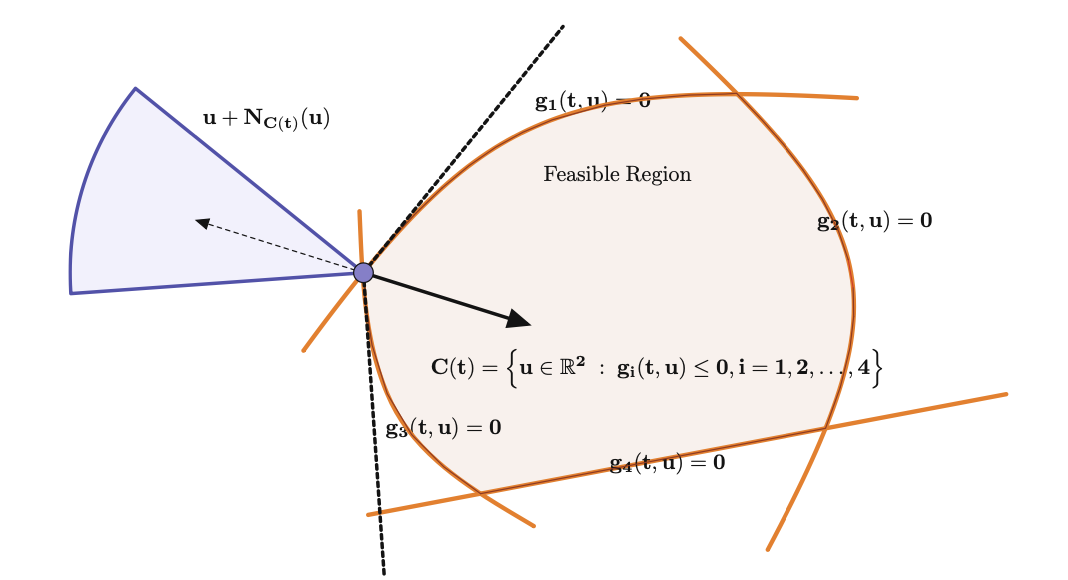
\includegraphics[width=0.5\linewidth]{swept_by_set.png}
        \caption{The point $x(t)$ is swept inward by $C(t)$}
        \label{fig:enter-label}
    \end{figure}    
\end{frame}

\begin{frame}{Example - the Prandtl-Reuss Elastoplastic model}
    \begin{itemize}
        \item A material is said to be elastic if it can return to its original shape after an external deformation. Alternatively, a material is said to have plasticity property if it permanently deforms under the application of an external force. Most materials are a combination of elastic and plastic.
        \item The strain in a material represents the ratio of change in dimension of an object to its original dimension. The stress gives us an idea of the amount of force acting per unit area on the body. For an $n$-dimensional object, the stress and strain are symmetric $n\times n$ tensors/matrices.
        \item The strain tensor can be modeled as $\epsilon^e + \epsilon^p$, where $\epsilon^e$ is the elastic strain, and $\epsilon^p$ is the plastic strain.
        \item The elastic strain is linearly related to the stress, $\sigma$, as $\epsilon^e = A^2\cdot \sigma$, where $A$ is a constant $n\times n$ symmetric P.D matrix (Hooke's law).
        \item The set of allowed stress tensors is a closed, convex subset $Z \subset symm(R^{n\times n})$, with $int(Z) \neq \phi$. That is $\sigma(t) \in Z \text{, } \forall \text{ }$ ($Z$ usually arises due to material constraints, like breaking point, contact with other surfaces etc).
    \end{itemize}
    
\end{frame}

\begin{frame}[fragile]{The Prandtl-Reuss Elastoplastic model}
    \begin{block}{Principle of maximum energy dissipation}
        Among all possible stress responses that are allowed by the material constraints, the one that occurs dissipates the maximum energy out of the object.
    \end{block}
    \begin{itemize}
        \item The rate of energy dissipated per unit volume is given by $\langle \dot{\epsilon}^p, \sigma\rangle$. Principle of maximum dissipation gives us $\langle \dot{\epsilon}^p(t), \sigma(t) \rangle \geq \langle \dot{\epsilon}^p(t), v\rangle \text{ } \forall \text{ } v \in Z$.
        \item Writing $\dot{\epsilon}^p = \dot{\epsilon} - A^2 \dot{\sigma}$ and rearranging terms give us $\langle \dot{\epsilon}(t) - A^2 \dot{\sigma}(t), v - \sigma(t) \rangle \leq 0 \text{, } \forall \text{ } v \in Z$. 
        \item Define $x(t) = A \sigma(t) - A^{-1}\epsilon(t)$, and $C(t) = A\cdot (Z) - A^{-1} \epsilon(t) = \{Av : v \in Z \} - A^{-1}\epsilon(t)$. The above equation can then be recast as $\langle -\dot{x}(t), p - x(t)\rangle \leq 0$ for all $p \in C(t)$, with $x(t) \in C(t) \text{ } \forall \text{ } t$ (this simply follows from the fact that $\sigma(t) \in Z$ for all t). This can be written as : 
            \begin{equation*}
                \begin{cases}
                    \dot{x}(t) \in -N(C(t); x(t))\\
                    x(t) \in C(t) \ \forall \ t
                \end{cases}
            \end{equation*}
    \end{itemize}
\end{frame}

\section{Math preliminaries}

\begin{frame}{Math preliminaries - recap}
    \begin{itemize}
        \item \textbf{\underline{Normal cone:}} The (outward) normal cone to a set $S\subset \mathbb{R}^n$ at a point $x \in S$, denoted $N(S; x)$ is defined as :
            \begin{equation*}
                N(S; x) = \{ w \in \mathbb{R}^n : \langle w, y-x\rangle \leq 0 \ \forall \ y \in S \}
            \end{equation*}
        \item \textbf{\underline{Distance of a point to a set}} : The distance between a point $x$ and a closed set $S$ is defined as $d_S(x) = \min_{y\in S}||x-y||$ (minima is well defined, thanks to closedness of $S$).
        \item \textbf{\underline{Projection onto a set :}} The projection of a point $x$ to a closed set $S$, denoted $proj_S(x)$ is the set of points in $S$ that are closest to $x$. That is, 
        \begin{align*}
            proj_S(x) = \{y\in S : ||y-x|| = d_S(x)\}
        \end{align*}
        The line joining a point $x$ to $proj_S(x)$ lies in the normal cone to $S$ at $proj_S(x)$.
        \begin{figure}[h]
            \centering
            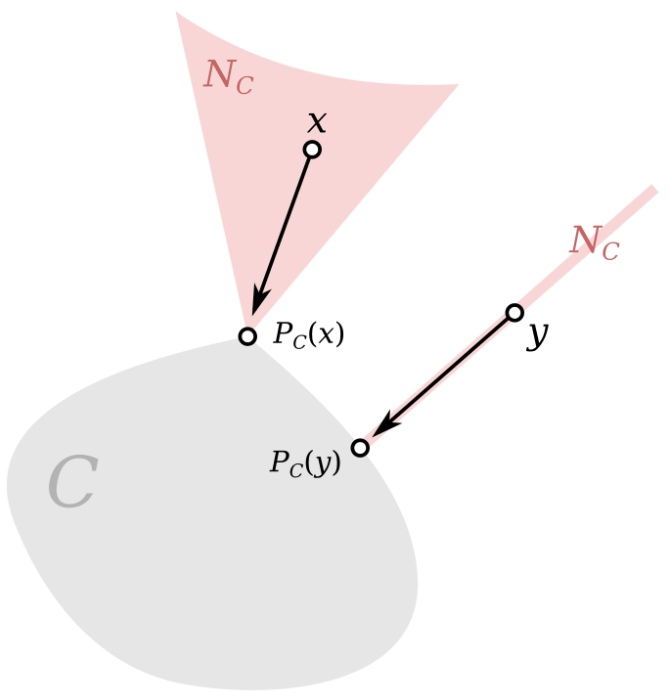
\includegraphics[width=0.2\linewidth]{projection.png}
            \caption{Projection onto a set and normal cone}
            \label{fig:enter-label}
        \end{figure}
    \end{itemize}
    
\end{frame}

\begin{frame}{Math preliminaries}
    \begin{itemize}
        \item \textbf{\underline{Cauchy sequences and convergence :}} A sequence $\{a_n\}$ defined on a metric is said to be Cauchy if for all $\epsilon > 0$, we can find an $N \in \mathbb{N}$ such that $||a_m - a_n|| \leq \epsilon \ \forall \ m,n \geq N$. \\

        A metric space is said to be complete if every Cauchy sequence converges. For eg, $\mathbb{R}$ is complete, but $\mathbb{Q}$, the set of rationals, is not.

        \begin{figure}[h]
            \centering
            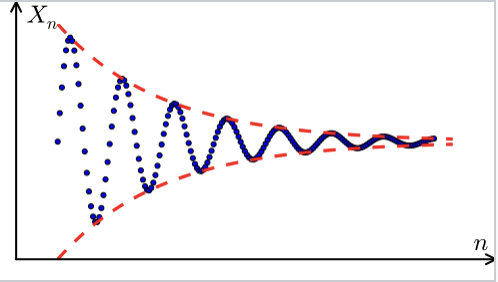
\includegraphics[width=0.2\linewidth]{cauchy_seq.png}
            \caption{Example of a Cauchy sequence}
            \label{fig:enter-label}
        \end{figure}

        \item \textbf{\underline{Lipschitz continuity :}} A function $f : \mathbb{R}^m \to \mathbb{R}^n$ is said to be L-Lipschitz continuous at a point $x$ if there exists a neighborhood $N$ of $x$ such that :
            \begin{align*}
                ||f(y) - f(z)|| \leq L\cdot ||y-z|| \ \forall \ y, z \in N
            \end{align*}

        \begin{block}{Theorem : Convergence of sequence of Lipschitz continuous functions}
        If $f_n(x)$ are a sequence of $L$-Lipschitz function such that $f_n$ converges to $f$ pointwise, then $f$ is also L-Lipschitz continuous.
    \end{block}
    \end{itemize}    
\end{frame}

\begin{frame}[fragile]{Math Preliminaries (contd.)}
    \begin{block}{Proof of theorem}
        We have $||f_n(x) - f_n(y)|| \leq L||x-y||$ for all $x, y$. Further,
        \begin{align*}
            ||f(x) - f(y)|| = ||\lim_{n\to\infty} f_n(x) - \lim_{n\to\infty}f_n(y)|| = \lim_{n\to \infty}||f_n(x) - f_n(y)|| \leq L||x-y||
        \end{align*}
        Thus, $f$ is also $L$-Lipschitz continuous.
        
    \end{block}
    \begin{itemize}
        \item \textbf{\underline{Almost everywhere and sets of measure 0 :}} A property $P$ is said to hold almost everywhere on a set $E$, if there exists a subset $N \subset E$ such that $\mu(N) = 0$, and $P$ holds for all points in $E-N$, where $\mu(.)$ is any measure on our underlying space.

        \item We will be working in $\mathbb{R}$, where $\mu(.)$ is the so-called Lebesgue measure - a generalization of length of an interval. Any collection of finite number of points (eg, $\{1, 2, \pi\}$) and any countable collection of points (the set of integers, rational numbers etc.) have measure 0.
    \end{itemize}
\end{frame}

\begin{frame}[fragile]{The Hausdorff distance}
    \begin{block}{Definition : Hausdorff distance between two sets}
        Let $A$ and $B$ be two closed sets in a metric space. The Hausdorff distance between $A$ and $B$, denoted $\text{Haus}(A, B)$ is defined as : 
        \begin{equation*}
            \text{Haus}(A, B) = \max \left\{ \sup_{x \in A} d_B(x), \sup_{y \in B} d_A(y) \right \},
        \end{equation*}
        where $d_S(p)$ denotes the distance between $p$ to its Euclidean projection on $S$, $proj_S(p)$.
    \end{block}

    \begin{itemize}
        \item The Hausdorff distance gives us an idea of how similar/dissimilar two sets are. If the Hausdorff distance between two sets is small, then they are 'not too far off'.
    \end{itemize}

    \begin{figure}[h]
        \centering
        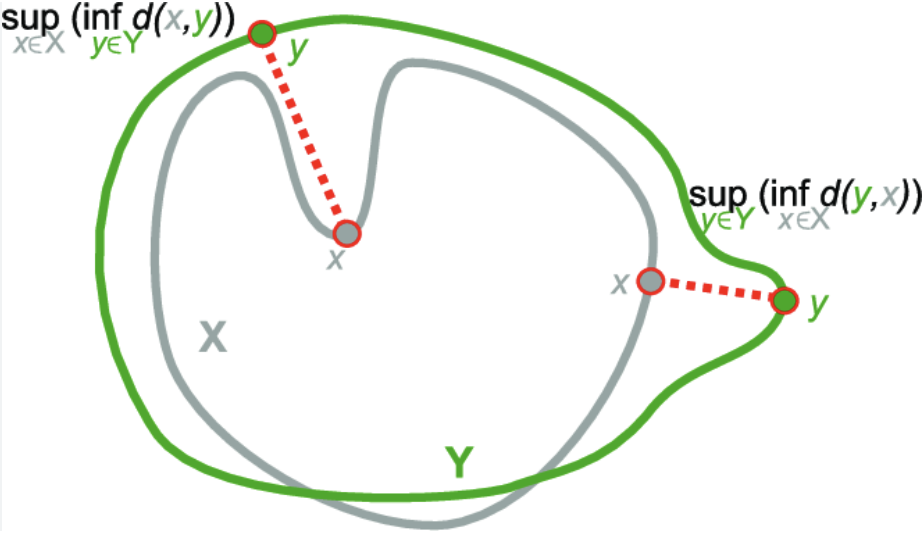
\includegraphics[width=0.25\linewidth]{haus.png}
        \caption{Hausdorff distance between two sets}
        \label{fig:enter-label}
    \end{figure}   
\end{frame}

\begin{frame}[fragile]{Properties of the Hausdorff distance}
    \begin{itemize}
        \item $Haus(A, B) = 0$ if and only if $A = B$.
        \item For any four sets $A_1, A_2, B_1, B_2$, we have: $$\text{Haus}(A_1 \cup A_2, B_1 \cup B_2) \leq \max \left \{\text{Haus}(A_1, B_1), \text{Haus}(A_2, B_2) \right \}$$.
    \end{itemize}
    \begin{block}{Proof of property 2}
        \begin{itemize}
            \item For a set $S\subset \mathbb{R}^n$ and $\epsilon > 0$, define the set $S_{\epsilon} = \{x\in \mathbb{R}^n : d_S(x) \leq \epsilon \}$.
            \item Let $r = \max \{\text{Haus}(A_1, B_1), \text{Haus}(A_2, B_2)\}$. Then, $A_i \subseteq (B_i)_r$ and $B_i \subseteq (A_i)_r$ for $i = 1, 2$.
            \item Therefore, $(B_1\cup B_2)_r = (B_1)_r \cup (B_2)_r \supset A_1 \cup A_2$. Similarly, $B_1\cup B_2 \in (A_1\cup A_2)_r$, which gives us $\text{Haus}(A_1\cup A_2, B_1\cup B_2)\leq r$.  
        \end{itemize}      
    \end{block}
    \begin{itemize}
        \item For any two closed sets $A$, $B$, $Haus(conv(A), conv(B)) \leq Haus(A, B)$, where $conv(.)$ denotes the convex hull operator.
    \end{itemize}
\end{frame}

\begin{frame}{Properties of the Hausdorff distance (contd.)}
    \begin{block}{Proof of property 3}
        \begin{itemize}
            \item Let $x \in conv(A)$. Then, $\exists \ a_1, \cdots a_n \in A$ such that $x = \sum_{i=1}^n \lambda_i a_i$ where $\lambda_1\geq 0$ and $\sum_{i=1}^n \lambda_i = 1$.
            \item By the definition of Hausdorff metric, for any $a\in A$, we have $d_B(a) \leq Haus(A, B)$. Thus, for each $a_i$, there exists a point $b_i \in B$ such that $||a_i - b_i|| \leq Haus(A, B)$.
            \item Let $y = \sum_{i=1}^n \lambda_i b_i$. Then, $y\in conv(B)$, and :
            \begin{align*}
                ||x - y|| = \left\vert \left\vert\sum_{i=1}^n \lambda_i\cdot(a_i - b_i) \right\vert \right\vert \leq \sum_{i=1}^n \lambda_i ||a_i - b_i|| \leq \sum_{i=1}^n \lambda_i\cdot Haus(A, B) = Haus(A, B)
            \end{align*}
            \item This means, for any point $x \in conv(A)$, there exists a point $y \in conv(B)$ such that $||x-y|| \leq Haus(A, B)$. This means, $d_{conv(B)}(x) = \min_{z\in conv(B)}||x-z|| \leq ||x-y|| \leq Haus(A, B)$. 
            \item Since $d_{conv(B)}(x) \leq Haus(A, B)$ for any point $x$ in $conv(A)$, we have :
            \begin{align*}
                \sup_{x \in conv(A)} d_{conv(B)}(x) \leq Haus(A, B)
            \end{align*}
            \item A similar argument, exchanging the roles of $A$ and $B$ gives us : $\sup_{y \in conv(B)} d_{conv(A)}(y) \leq Haus(A, B)$
            \item Combining the above two inequalities finally gives us $Haus(conv(A), conv(B)) \leq Haus(A, B)$.
        \end{itemize}        
    \end{block}    
\end{frame}

\begin{frame}[fragile]{Monotone set valued operator}
    Let $F : \mathbb{R}^n \rightrightarrows \mathbb{R}^n$ be a set valued map. The graph of $F$ is all the points of the form $(x, u)$ where $u \in F(x)$. The map $F$ is said to be monotone, if for all $(x, u)$ and $(y, v)$ in the graph of $F$ (sometimes also denoted as $(x, u), (y, v) \in F$), we have : 
    \begin{align*}
        \langle u-v, x-y \rangle \geq 0
    \end{align*} 
    
    \begin{figure}[h]
     \centering
     \begin{subfigure}[b]{0.4\textwidth}
         \centering
         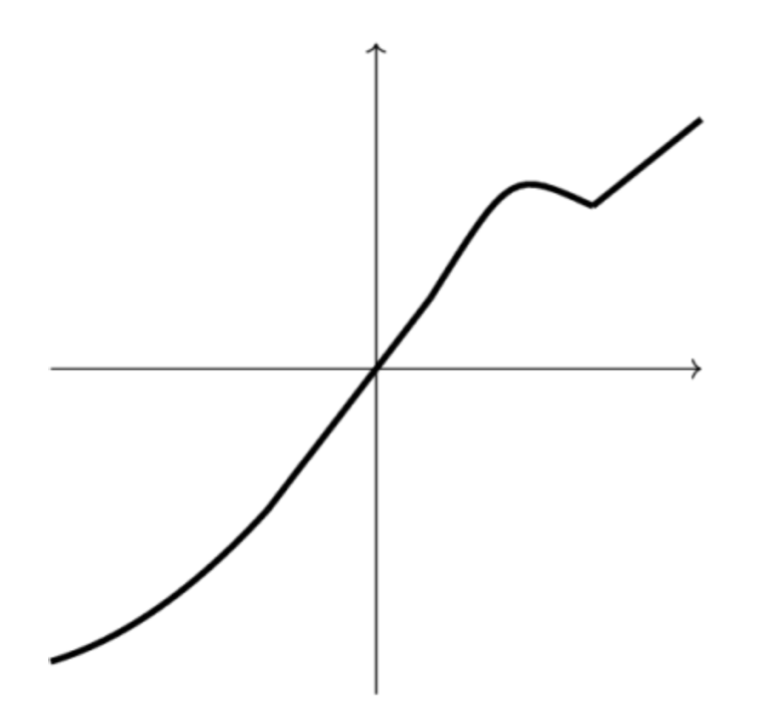
\includegraphics[width=0.3\textwidth]{nonmono.png}
         \caption{Non-monotone map}
         \label{fig:y equals x}
     \end{subfigure}
     \hfill
     \begin{subfigure}[b]{0.4\textwidth}
         \centering
         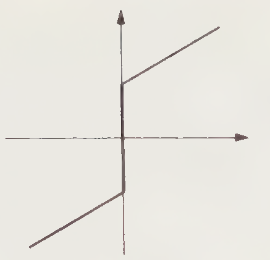
\includegraphics[width=0.3\textwidth]{monotone.png}
         \caption{Monotone set valued map}
         \label{fig:three sin x}
     \end{subfigure}

     \begin{block}{The subdifferential is a monotone operator}
        Let $f$ be a convex function and $u \in  \partial f(x)$ and $v \in \partial f(y)$. Then, $f(y) - f(x) \geq \langle u, y-x\rangle$ and $f(x) - f(y) \geq \langle v, x - y \rangle$. Adding these two inequalities give us $0 \geq \langle u-v, y-x\rangle$ or $\langle u-v, x -y \rangle \geq 0$.\\
         
     \end{block}

     $N(C; x)$, which is the subdifferential of $I_C(x)$ is therefore a monotone operator.
\end{figure}
\end{frame}

\begin{frame}[fragile]{Resolvent of an operator}
    Let $F$ be a set valued map, and let $\lambda \in \mathbb{R}$. The resolvent of $F$ (w.r.t $\lambda$) is defined as the inverse relation $(I + \lambda F)^{-1}$, where $I$ is the identity map. That is, 
    \begin{align*}
        I + \lambda F = \{(x, x+\lambda y) : (x, y) \in F\}\\
        (I + \lambda F)^{-1} = \{(x+\lambda y, x) : (x, y) \in F\}
    \end{align*}

    \begin{block}{Resolvent for the subdifferential operator}
        Let $f$ be a convex function, and let $\lambda > 0$. Let $z \in (I + \lambda \partial f)^{-1} (x)$. This means $x \in z + \lambda \partial f(z)$. Or equivalently, $0 \in (z-x) + \lambda \partial f(z)$. This is same as : 
    \begin{align*}
        0 \in \left. \partial \left( f(u)  + \frac{1}{2\lambda} ||u-x||_2^2 \right)\right \vert_{u=z}
    \end{align*}

    This means $z$ is a minimizer for the regularized function $f(u) + \frac{1}{2\lambda}||u-x||^2$. And since $f$ is convex and $||u-x||^2$ is strictly convex, their sum is strictly convex, so $z$ is the unique minimizer. Thus, $z = \text{arg min}_u f(u) + \frac{1}{2\lambda}||u-x||^2$. This is sometimes also called the proximal mapping of $f$ (w.r.t $\lambda$), i.e $z = \text{prox}_{\lambda f}(x)$. \textcolor{violet}{The resolvent for the subdifferential operator is a singleton map}.\\
    
    When we take $f = I_C$, we will have $\partial f = N_C$. And $\text{arg min}_u I_C(u) + \frac{1}{2\lambda}||u-x||^2$ is simply the projection of $x$ onto the set $C$, thus we have $(I + \lambda N_C)^{-1}(x) = \text{proj}_C(x)$.
        
    \end{block}
\end{frame}

\section{The classical sweeping process}

\begin{frame}[fragile]{Solution to the classical sweeping process}
    A main bottleneck in constructing solution to the sweeping process (eq. \ref{swp}) is that it has the constraint $x(t) \in C(t) \ \forall \ t$. What we have is not a regular differential inclusion, but a constrained one. 
    

    The following existence result was stated and proven by Moreau, around the year 1971.

    \begin{block}{Theorem : Existence and uniqueness of solution to the sweeping process (Moreau, 1971)}
        If the sets $(C(t))_{t\geq 0}$ are nonempty, closed and convex with :
    \begin{align*}
        \text{Haus}(C(t), C(s)) \leq k\cdot |t-s|
    \end{align*}
    for some $k \geq 0$ and for all $t, s\in [0, T]$, then there exists a \textbf{unique} Lipschitz continuous solution for the sweeping process :
    \begin{align*}
        \begin{cases}
            \dot{x}(t) \in -N(C(t); x(t)) \text{ a.e } t \in [0, T]\\
            x(0) = x_0 \in C(0)\\
            x(t) \in C(t) \text{, } \forall \text{ } t \in [0, T]
        \end{cases}
    \end{align*}
    Moreover, $||\dot{x}(t)|| \leq k$ a.e on $[0, T]$.
        
    \end{block}

    $\text{Haus}(C(t), C(s)) \leq k\cdot |t-s|$ ensures that the movement of $C(t)$ is well-behaved and does not have sudden movements. This ensures existence of solution.
\end{frame}

\begin{frame}{Proof - The 'Catching-up' Algorithm}
    \begin{itemize}[<+->]
        \item Let $\{t_0^n, t_1^n, t_2^n, \cdots, t_n^n\} = \{0, t_1^n, t_2^n, \cdots, T\}$ be a partition of the interval $[0, T]$. For $0 \leq i \leq n-1$ define the interval $I_i^n = (t_i^n, t_{i+1}^n]$. Discretize our differential inclusion over every $I_i^n$ by using $\{t_i^n\}$ as sampling times : 
            \begin{align*}
                \dot{x}(t) \approx \frac{x(t_{i+1}^n) - x(t_i^n)}{t_{i+1}^n - t_i^n} \in -N(C(t); x(t)) \approx -N\left (C(t_{i+1}^n), x(t_{i+1}^n)\right )
            \end{align*}
        \item This gives $x(t_{i+1}^n) - x(t_i^n) \in -N(C(t_{i+1}^n), x(t_{i+1}^n))$, or $x(t_i^n) \in (I+ N(C(t_{i+1}^n); .)\ )(x(t_{i+1}^n))$. 
        \item Rewrite this as $x(t_{i+1}^n) = (I+ N(C(t_{i+1}^n); .)\ )^{-1}(x(t_i^n)) = proj_{C(t_{i+1}^n)}(x(t_i^n))$ (recall that the resolvent for the normal cone is the projection operation).
        \item This update rule forms the basis for our catching-up algorithm :
            \begin{align*}
                \begin{cases}
                    x(t_{i+1}^n) = proj_{C(t_{i+1}^n)}(x(t_i^n)) \ \textbf{, catching-up algorithm}\\
                    x(0) = x_0 \in C(0)
                \end{cases}
            \end{align*}
        \item $x_i^n$ catches up to $C(t)$ by projecting itself onto the place where $C(t)$ will be next. $x_i^n$ is 'lazy' since it moves the least distance it can to ensure it stays in $C(t)$. 
    \end{itemize}
\end{frame}

\begin{frame}{The Catching-up algorithm}
    \begin{figure}
        \centering
        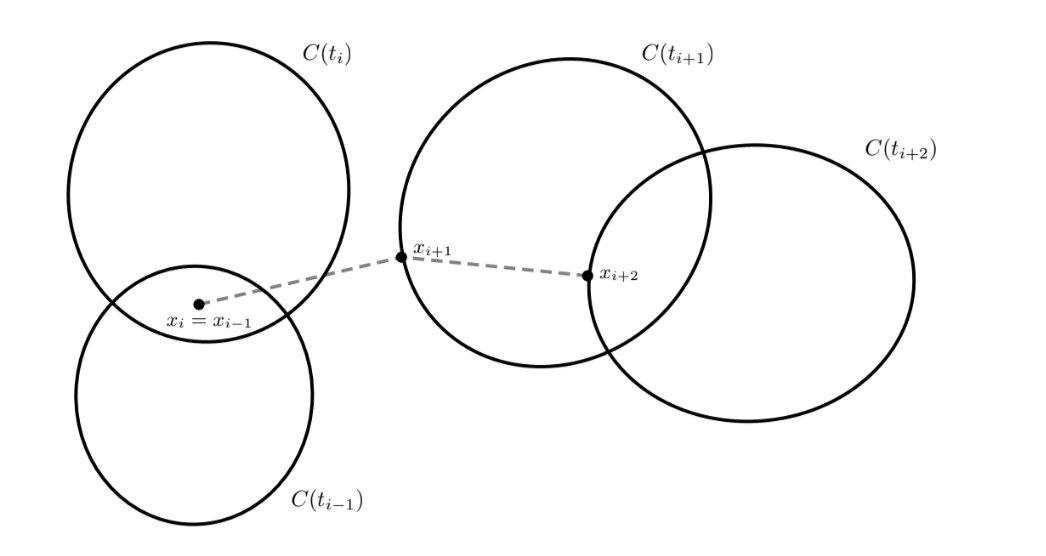
\includegraphics[width=0.35\linewidth]{catch_up.png}
        \caption{The catching-up algorithm}
        \label{fig:enter-label}
    \end{figure}
    \begin{itemize}
        \item Define for every $n \in \mathbb{N}$, the following sequence of functions : 
            \begin{align*}
                x_n(t) = \begin{cases}
                x_0, \text{ if } t = 0\\
                x_i^n + \frac{t - t_i^n}{t_{i+1}^n - t_i^n}\cdot (x_{i+1}^n - x_i^n), \text{ if } t \in I_i^n,  0\leq i \leq n-1
                \end{cases}
            \end{align*}
        \item Its easy to see that $x_n(t)$ is a continuous function and is differentiable in the interior of each interval $I_i^n$. Thus, $x_n(t)$ is differentiable a.e on $[0, T]$.
    \end{itemize}
\end{frame}

\begin{frame}[fragile]{The Catching-Up algorithm - properties of $x_n(t)$}
    \begin{itemize}
        \item Whenever $x_n(t)$ is differentiable, we also have $||\dot{x}_n(t)|| \leq k$. That is, $||\dot{x}_n||\leq k$ a.e on $[0, T]$.
    \end{itemize}
    \begin{block}{Why is $||\dot{x}_n||\leq k$?}
        We have $||\dot{x_n}(t)|| = \frac{||x_{i+1}^n - x_i^n||}{t_{i+1^n - t_i^n}}$, from the piecewise definition of $x_n(t)$. By definition of our update rule, we have $x_i^n \in C(t_i^n)$ for all $i$. The numerator of the RHS is $||\text{proj}_{C(t_{i+1}^n)}(x_i^n) - x_i^n||$. We then have :
    \begin{align*}
        ||\text{proj}_{C(t_{i+1}^n)}(x_i^n) - x_i^n|| \leq \max_{x \in C(t_i^n)} ||\text{proj}_{C(t_{i+1}^n)}(x) - x|| \leq \text{Haus}(C(t_{i+1}^n), C(t_i^n)) \leq k\cdot (t_{i+1}^n - t_i^n)
    \end{align*}
    So, $||x_{i+1}^n - x_i^n|| \leq k(t_{i+1}^n - t_i^n)$, and this gives us $||\dot{x}_n(t)|| \leq k$ for all points in the interior of $I_i^n$. Thus, $||\dot{x_n}(t)|| \leq k $ a.e on $[0, T]$.
    \end{block}

    \begin{itemize}
        \item As $x_n(t)$ is a piecewise affine function, it is Lipschitz continuous. And since $||\dot{x}_n(t)||\leq k$ a.e, it is $k$-Lipschitz continuous.
    \end{itemize}
\end{frame}

\begin{frame}[fragile]{The Catching-up Algorithm - convergence of $x_n$}
    \begin{block}{The sequence of functions $x_n$ is Cauchy, and hence converges to a continuous function $x(t)$}
        \begin{itemize}
            \item Consider $x_n(t)$ and $x_m(t)$ ($m, n \in \mathbb{N}$). Let $t \in (t_i^n, t_{i+1}^n]$ as well as in $(t_j^m, t_{j+1}^m]$.
            \item Then, $x_n(t) \in conv(x_i^n\cup x_{i+1}^n)$, and $x_m(t) \in conv(x_j^m\cup x_{j+1}^m)$. We have $Haus(conv(x_i^n\cup x_{i+1}^n), conv(x_j^m\cup x_{j+1}^m)) \leq Haus(\{x_i^n\}\cup\{x_{i+1}^n\}, \{x_j^m\}\cup\{x_{j+1}^m\}) \leq \max\{||x_i^n - x_j^m||, ||x_{i+1}^n - x_{j+1}^m||\}$.
            \item As $m,n \to \infty$, the RHS goes to 0, and this means the line segments in which $x_n$ and $x_m$ reside are the same. 
            \item This means $d(x_n(t), x_m(t)) \leq d(x_i^n, x_{i+1}^n)$ (distance between 2 points in a line segment vs distance between end points of line segment). 
            \item The RHS is $||x_i^n - proj_{C(t_{i+1}^n)}x_{i}^n|| \leq Haus(C(t_i^n), C(t_{i+1}^n)) \leq k\cdot |t_{i+1}^n - t_i^n|$ which $ \to 0$ as $n \to \infty$
            \item So the sequence $x_n$ is Cauchy, and therefore converges to a function $x$.
        \end{itemize}   
    \end{block}
    As each $x_n(t)$ is k-Lipschitz continuous, the limit $x(t)$ is also $k$-Lipschitz continuous.
\end{frame}

\begin{frame}{The Catching-up algorithm - Differential inclusion model for $x_n(t)$}
    \begin{itemize}
        \item From the definition of $x_n(t)$, we have $\dot{x}_n = \frac{x_{i+1}^n - x_i^n}{t_{i+1}^n - t_i^n}$ a.e on $[0, T]$. As $x_{i+1}^n = proj_{C(t_{i+1}^n)}(x_i^n)$, we have $x_i^n - x_{i+1}^n \in N(C(t_{i+1}^n; x_{i+1}^n))$ (since the line joining a point to its projection lies in the normal cone at the projected point). This gives $\dot{x}_n(t) \in -N(C(t_{i+1}^n); x_{i+1}^n)$ a.e on $[0, T]$.
        \item Define for all $t \in [0, T]$ the function $\theta_n(t)$ as follows : 
            \begin{align*}
                \theta_n(t) = \begin{cases}
                0, \text{ if } t = 0\\
                t_{i+1}^n, \text{ if } t \in I_i^n \text{ for } 0 \leq i \leq n-1
                \end{cases}
            \end{align*}
        \item This allows us to rewrite the differential inclusion for $x_n(t)$ as :
        \begin{align}\label{DI}
            \begin{cases}
            \dot{x}_n(t) \in -N(C(\theta_n(t)); x_n(\theta_n(t))) \text{ a.e on } t \in [0, T]\\
            x_n(0) = x_0 \in C(0)
            \end{cases}
        \end{align}
    \end{itemize}
\end{frame}

\begin{frame}{The Catching-up Algorithm - refinement of partitions}
    \begin{itemize}[<+->]
        \item It can be proven that $\dot{x}_n$ (weakly) converges to $\dot{x}$ (this mainly uses the fact that $||\dot{x}_n||$ is bounded by $k$, therefore it is compact in the $L^\infty$ space).
        \item Letting $n\to \infty$ (refinement of partition of the interval $[0, T]$, and using $\dot{x}_n \to \dot{x}$, $x_n \to x$, $\theta_n(t) \to t$ in eq. \ref{DI}, we finally get : 
        \begin{align*}
            \begin{cases}
           \dot{x}(t) \in -N(C(t); x(t)) \text{ a.e on } t \in [0, T]\\
            x(0) = x_0 \in C(0) 
            \end{cases}
        \end{align*}
        \item It remains to show that $x(t) \in C(t) \ \forall \ t \in [0, T]$.
    

        \item Let $t \in (t_i^n, t_{i+1}^n]$. Then, by definition, $x_n(t) = x_i^n + \frac{t - t_i^n}{t_{i+1}^n - t_i^n}\cdot x_{i+1}^n \in conv(C(t_i^n) \cup C(t_{i+1}^n))$. So, $d(C(\theta_n(t)); x_n(t)) = d(C(t_{i+1}^n); x_n(t)) \leq Haus(C(t_{i+1}^n), conv(C(t_i^n) \cup C(t_{i+1}^n)))$.
        \item Since $C(t)$ is closed and convex, $C(t_{i+1}^n) = conv(C(t_{i+1}^n) \cup C(t_{i+1}^n))$. This gives $d(C(\theta_n(t)); x_n(t))) \leq Haus(conv(C(t_{i+1}^n) \cup C(t_{i+1}^n)), conv(C(t_i^n) \cup C(t_{i+1}^n))) \leq Haus(C(t_{i+1}^n) \cup C(t_{i+1}^n), C(t_i^n) \cup C(t_{i+1}^n))$
        \item The final term in RHS is less than or equal to $Haus(C(t_{i+1}^n), C(t_i^n)) \leq k\cdot |t_{i_+1}^n - t_i^n|$. Letting $n \to \infty$ makes this zero, which gives us $d(C(t), x(t)) = 0$. Thus $x(t) \in C(t) \ \forall \ t \in [0, T]$. \textcolor{purple}{$x(t)$ is a solution!}
    \end{itemize}
\end{frame}

\begin{frame}[fragile]{Uniqueness of solution}
    \begin{block}{Uniqueness of solution}
        The solution $x(t)$ for the sweeping process (eq. \ref{swp}) is unique among the class of absolutely continuous functions.
    \end{block}
    
    \textbf{Proof : } Follows from the fact that the normal cone is a monotone operator.
    \begin{itemize}
        \item Let $u(t)$ be an absolutely continuous solution to $\dot{u} \in -N_{C(t)}(u(t))$ with the initial condition $u(0) = u_0$, and let $v(t)$ be an absolutely continuous solution to $\dot{v} \in -N_{C(t)}(v(t))$, with the initial condition $v(0) = v_0$.
        \item As $u$ and $v$ are absolutely continuous, we have : 
            \begin{align*}
            \frac{d}{dt} \left(\frac{1}{2} ||u(t) - v(t)||^2\right) = \langle \dot{u} - \dot{v}, u-v \rangle \text{ a.e on } t \in (0, T)
            \end{align*}
        \item $u(t)$ and $v(t)$ are points in $C(t)$, and from our differential inclusion model,  $-\dot{u} \in N_{C(t)}(u(t))$ and $-\dot{v} \in N_{C(t)}(v(t))$. Using the fact that the normal cone is a monotone operator $\langle \dot{u} - \dot{v}, u-v \rangle \leq 0$ a.e on $(0, T)$. Integration then yields :
        \begin{align*}
            ||u(t) - v(t)||^2 \leq ||u(0) - v(0)||^2 \text{ for all } t\in [0, T]
        \end{align*}
        \item Setting $u(0) = v(0)$ then guarantees uniqueness (since $||u(t) - v(t)||^2 = 0$ for all time).
    \end{itemize}
\end{frame}

\begin{frame}{Simulation}
    \begin{itemize}
        \item The catching-up algorithm allows for an explicit construction of solution.
        \item Below is a simulation where $C(t)$ is a square of side length 2, whose center moves in the parabola $(t, t^2)$, and rotates with a constant angular speed of $15^\circ$ per sec. The point $x(t)$ starts from the upper left corner $(-1, 1)$ and tracks the moving square.
    \end{itemize}
    \centering
    \animategraphics[autoplay, loop, width = 0.35\textwidth]{10}{frames/frame_}{000}{059}
\end{frame}

\section{The perturbed sweeping process}

\begin{frame}{Example - crowd motion}
    \begin{itemize}
        \item Consider $N$ persons modeled as rigid, non-overlapping discs of radius $r$ in $\mathbb{R}^2$, and lets say each person wants to immediately evacuate to the exit. 
        \item Let the center of the $i^{th}$ person's disc be at $q_i \in \mathbb{R}^2$. Let the collective coordinates of all the centers be $\boldsymbol{q} = (q_1, q_2, \cdots q_N) \in \mathbb{R}^n$.
        \item Since each person is modeled as rigid, non-overlapping discs, the set of feasible coordinates is defined by :
        \begin{align*}
            Q = \{\boldsymbol{q} \in \mathbb{R}^{2N} : D_{ij}(\boldsymbol{q})\geq 0 \ \forall \ i
        \leq j\},
        \end{align*}
        where $D_{ij}(\boldsymbol{q}) = ||q_i - q_j|| - 2r$, the signed distance between disks $i$ and $j$.
    \end{itemize}

    \begin{figure}[h]
        \centering
        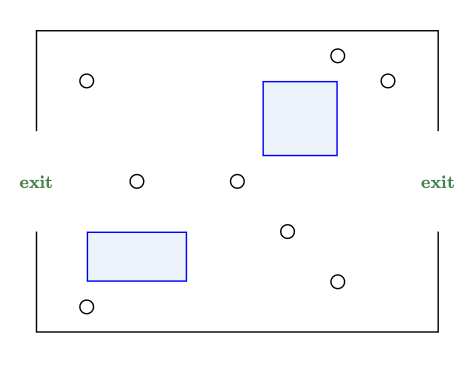
\includegraphics[width=0.26\linewidth]{crowd.png}
        \caption{Each person wants to escape via the nearest exit}
        \label{fig:enter-label}
    \end{figure}    
\end{frame}

\begin{frame}{Crowd motion (contd.)}
    \begin{itemize}
        \item The spontaneous velocity of all the agents is given by $U(\boldsymbol{q}) = (u_1(\boldsymbol{q}), u_2(\boldsymbol{q}), \cdots, u_N(\boldsymbol{q})) \in \mathbb{R}^{2N}$ - this is the set of velocities each agent \textbf{would like to take}.
        \item The set of feasible velocities is given by : $C(q) = \{v \in \mathbb{R}^{2N}: \ \forall \ i<j \text{ s.t } D_{ij}(\boldsymbol{q}) = 0, G_{ij}(\boldsymbol{q})\cdot v \geq 0\}$, where $G_{ij}(\boldsymbol{q}) = \nabla D_{ij}(\boldsymbol{q}) = (0, \cdots, 0, -e_{ij}(\boldsymbol{q}), 0, \cdots, e_{ij}(\boldsymbol{q}), \cdots, 0) \in \mathbb{R}^{2N}$, and $e_{ij}(\boldsymbol{q}) = \frac{q_j - q_i}{||q_j - q_i||}$.
        \item Intuitively, the set of feasible velocities tells that if two balls are in contact, then they must have a non-negative velocity of separation.
    \end{itemize}
    \begin{figure}[h]
        \centering
        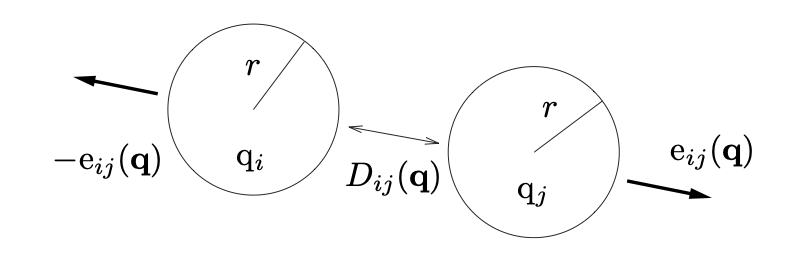
\includegraphics[width=0.4\linewidth]{separation.png}
        \caption{Depiction of $e_{ij}$ and $D_{ij}$}
        \label{fig:enter-label}
    \end{figure}
    \begin{itemize}
        \item So the actual velocity taken by the particles is the projection of the spontaneous velocity onto the set of feasible velocities.
    \end{itemize}
\end{frame}

\begin{frame}{Crowd motion - recasting the model}
    \begin{itemize}
        \item The motion of the agents is modeled by the projected dynamical system : 
        \begin{align*}
            \begin{cases}
                \frac{d\boldsymbol{q}}{dt} = proj_{C(q)}(U(\boldsymbol{q}))\\
                \boldsymbol{q}(0) = \boldsymbol{q}_0 \in Q
            \end{cases}
        \end{align*}
        \item The feasible set is given by $Q = \{\boldsymbol{q} \in \mathbb{R}^{2N} : D_{ij}(\boldsymbol{q})\geq 0 \ \forall \ i
        \leq j\}$, and the set of feasible velocities is $C(q) = \{v \in \mathbb{R}^{2N}: \ \forall \ i<j \text{ s.t } D_{ij}(\boldsymbol{q}) = 0, \nabla D_{ij}(\boldsymbol{q})\cdot v \geq 0\}$. This is precisely the set of feasible directions to $Q$ at $\boldsymbol{q}$. Since the gradients of the active constraints are linearly independent, $C(q)$ is also the tangent cone to $Q$ at $\boldsymbol{q}$.
        \item So the normal cone to $Q$ is the polar of the cone of feasible velocities :
        \begin{align*}
            N(Q; \boldsymbol{q}) = C(q)^\circ = \{w\in \mathbb{R}^{2N} : \langle w, v\rangle \leq 0 \ \forall \ v \in C(q)\}
        \end{align*}
        \item Moreau's decomposition theorem says that the sum of projections onto a cone $K$, and its polar cone $K^\circ$ is simply the identity operator. That is, $proj_K(.) + proj_{K^\circ}(.) = I(.)$
    \end{itemize}

    \begin{figure}[h]
        \centering
        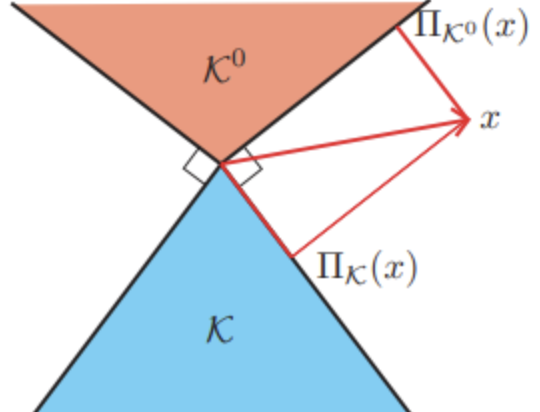
\includegraphics[width=0.15\linewidth]{decomp.png}
        \caption{Moreau's decomposition theorem/ two cones lemma}
        \label{fig:enter-label}
    \end{figure}
\end{frame}

\begin{frame}{Crowd motion - recasting the model (contd.)}
    \begin{itemize}
        \item The above theorem gives us $proj_{C(q)}(U(\boldsymbol{q})) = U(\boldsymbol{q}) - proj_{N(Q; \boldsymbol{q})}(U(\boldsymbol{q}))$.
        \item We can use this to remodel the differential equation as :
        \begin{align*}
            \begin{cases}
                \frac{d\boldsymbol{q}}{dt} = U(\boldsymbol{q}) - proj_{N(Q; \boldsymbol{q})}(U(\boldsymbol{q}))\\
                \boldsymbol{q}(0) = \boldsymbol{q}_0 \in Q
            \end{cases}
        \end{align*}
        \item The solution to the above projected dynamical system turns out to be the same as the minimum norm solution to the differential inclusion \footnote{Refer to : Dynamical systems coupled with monotone set-valued operators: Formalisms, applications, well-posedness, and stability, by Bernard Brogliato, Aneel Tanwani} - 
        \begin{align*}
            \begin{cases}
                \frac{d\boldsymbol{q}}{dt} \in U(\boldsymbol{q}) - N(Q; \boldsymbol{q})\\
                \boldsymbol{q}(0) = \boldsymbol{q}_0 \in Q
            \end{cases}
        \end{align*}
        \item The above example motivates the study of \textbf{perturbed sweeping process}, which are differential inclusions of the form : 
        \begin{align*}
            \begin{cases}
                -\dot{x}(t) \in N(C(t); x(t)) + F(t, x(t)) \ \text{a.e on } t \in [0, T]\\
                x(0) = x_0 \in C(0)
            \end{cases}            
        \end{align*}
        where $F(t, x(t))$, called the perturbation term, is a set valued map.
    \end{itemize}   
\end{frame}

\begin{frame}{Some definitions}
    \begin{itemize}
        \item A set valued map $\Omega : T \rightrightarrows X$ is said to be measurable if for every open set $B \in X$, the set $\Omega^{-1}(B) = \{t\in T : \Omega(t) \cap B \neq \phi\}$ is measurable in $T$.
        \item A set valued map $F : X \rightrightarrows Y$ is said to be upper semi-continuous at $x_0$ if for every open set $U \supset F(x_0)$, there exists a $\delta > 0$ such that :
        \begin{align*}
            F(B(x_0, \delta)) = \bigcup_{x\in B(x_0, \delta)} F(x) \subset U
        \end{align*}
        \item $F$ is said to be a Caratheodory set-valued map, if it is both measurable and u.s.c.
        \item Given a set $S$, the open $r$-tube centered at $S$, denoted $U_r(S)$ is defined as $\{x: 0 < d_S(x) < p\}$. Let $\alpha \in (0, 1]$ and $0 < r\leq \infty$. We say that the Clarke subdifferential of the distance function, $d_S(.)$ keeps the origin $\alpha$-far off on the open $r$-tube around $S$, if :
        \begin{align}\label{alphafar}
            0 < \alpha \leq \inf_{x \in U_r(S)} d_{\partial d(., S)(x)}(0)
        \end{align}
        \item The family of sets $(S(t))_{t\in E}$ ($E$ is any non-empty sets) is said to be \textbf{positively $\alpha$-far}, if for each $t\in E$, $S(t)$ satisfies \ref{alphafar}, for the same value of $\alpha$ and $r$.
    \end{itemize}    
\end{frame}

\begin{frame}[fragile]{Existence of solution to the perturbed sweeping process}
    \begin{block}{Theorem - existence of solution (Jourani and Vilches, 2017)} \footnote{A. Jourani, E. Vilches, Galerkin-like method and generalized perturbed sweeping process with nonregular sets, SIAM J. Control Optim., 55(4):2412-2436, 2017.}
        Assume the following assumptions hold true :
        \begin{itemize}
            \item $F$ is a Caratheodory set-valued map.
            \item The family $(C(t))_{t\in[0, T]}$ is positively $\alpha$-far.
            \item $Haus(C(t), C(s)) \leq k\cdot |t-s|$ for some $k\geq 0$ and for all $t, s \in [0, T]$.
        \end{itemize}
        Then, there exists at least one absolutely continuous solution of : 
        \begin{align*}
            \begin{cases}
                -\dot{x}(t) \in N(C(t); x(t)) + F(t, x(t)) \text{ a.e on } t\in [0, T]\\
                x(0) = x_0 \in C(0)
            \end{cases}
        \end{align*}
        \begin{itemize}
            \item The solution need not necessarily be unique when $C(t)$ is nonconvex, but uniqueness is guaranteed if $C(t)$ is convex.
        \end{itemize}
    \end{block}
\end{frame}


\section{Summary}

\begin{frame}{Summary}
	\begin{itemize}
		\item Seen the motivation for the Moreau's sweeping process, some example systems that can be modeled by the sweeping process.
        \item Covered some ideas that are key to the sweeping process, and proved existence and uniqueness results.
        \item A glimpse into a variant of the sweeping process, called the perturbed sweeping process. Stated a sufficient condition for existence of solution.
	\end{itemize}
\end{frame}

\begin{frame}{Future work and open problems}
    \begin{itemize}
        \item Sweeping process and its many variants (perturbed sweeping process, state-dependent sweeping process, implicit sweeping process, etc.) are very rich in theory, and can model a variety of real-life systems.
        \item Active research is still done in this field, and there are many fundamental questions left to answer, such as :
        \begin{enumerate}
            \item Existence and uniqueness of solutions - What happens when $C(t)$ is not well-behaved? Does a solution exist? Is it unique? More 'lenient' conditions for existence of solutions to the variants of the sweeping process? Uniqueness results?
            \item Stability and asymptotic behavior of the sweeping process and its variants - can we have equilibrium points for the sweeping process model? Are these stable? Can these be stabilized? Is it possible to observe limit cycles? 
            \item Optimal control of the sweeping process.
        \end{enumerate}
    \end{itemize}
\end{frame}
%\backmatter % generate the final slide
\end{document}
